%\documentclass[aps, reprint, notitlepage,  superscriptaddress, prl, onecolumn]{revtex4-1}
\documentclass[aps,amssymb,amsmath,prb,superscriptaddress,reprint,notitlepage,onecolumn]{revtex4-1}

\usepackage{blindtext}
\usepackage{graphicx}
\usepackage{xcolor}
\usepackage{amsmath}
\usepackage{amsthm}
\usepackage{amssymb}
\usepackage{amsfonts}
\usepackage{xr-hyper}
\usepackage{hyperref}
\usepackage{multirow}
\hypersetup{
    colorlinks,
    linkcolor={blue},
    citecolor={blue},
    urlcolor={blue}
}
\usepackage{siunitx}
\usepackage{bm}
\usepackage{xpatch}
\usepackage[normalem]{ulem}
\usepackage{comment}
\usepackage[caption=false]{subfig}
\usepackage{lineno}
\usepackage{physics}

\renewcommand{\theequation}{S\arabic{equation}}
\renewcommand{\thefigure}{S\arabic{figure}}

\newcommand{\matlab}{{\sc Matlab} }
\newcommand{\cvec}[1]{{\mathbf #1}}	
\newcommand{\rvec}[1]{\vec{\mathbf #1}}
\newcommand{\ihat}{\hat{\textbf{\i}}}
\newcommand{\jhat}{\hat{\textbf{\j}}}
\newcommand{\khat}{\hat{\textbf{k}}}
\newcommand{\minor}{{\rm minor}}
\newcommand{\spn}{{\rm Span}}
\newcommand{\rem}{{\rm rem}}
\newcommand{\ran}{{\rm range}}
\newcommand{\range}{{\rm range}}
\newcommand{\mdiv}{{\rm div}}
\newcommand{\proj}{{\rm proj}}
\newcommand{\R}{\mathbb{R}}
\newcommand{\N}{\mathbb{N}}
\newcommand{\rr}{\mathbf{r}}
\newcommand{\kk}{\mathbf{k}}
\newcommand{\Q}{\mathbb{Q}}
\newcommand{\Z}{\mathbb{Z}}
\newcommand{\<}{\langle}
\renewcommand{\>}{\rangle}

\newcommand{\LL}{\mathcal{L}}
\newcommand{\VV}{\mathcal{V}}
\newcommand{\kT}{k_\text{B}T}
\newcommand{\keps}{{\mathbf{k} \varepsilon}}
\newcommand{\vac}{\sqrt{\frac{\hbar \omega_\mathbf{k}}{2\varepsilon_0 \mathcal{V}}}}
\newcommand{\vacc}{\sqrt{\frac{\hbar \omega}{16\pi^3\varepsilon_0}}}
\newcommand{\therm}{\text{th}}
\newcommand{\inn}{\mathrm{in}}
\newcommand{\outt}{\mathrm{out}}
\newcommand{\intdk}{\int_{\mathbb{R}^3}\dd^3k\,}

% MR new commands
\newcommand{\blue}[1]{\textcolor{blue}{#1}}
\newcommand{\bcanc}[1]{{\blue{\sout{#1}}}}
\newcommand{\yellow}[1]{\textcolor{brown}{#1}}
\newcommand{\ycanc}[1]{{\yellow{\sout{#1}}}}
\newcommand{\red}[1]{\textcolor{red}{#1}}
\newcommand{\rcanc}[1]{{\red{\sout{#1}}}}
\newcommand{\green}[1]{\textcolor{green}{#1}}
\newcommand{\gcanc}[1]{{\green{\sout{#1}}}}
\newcommand{\magenta}[1]{\textcolor{magenta}{#1}}
\newcommand{\mcanc}[1]{{\magenta{\sout{#1}}}}

\newcommand{\imu}{\text{\rm i}}
\newcommand{\expu}{\text{\rm e}}
\newcommand{\Og}{\Omega}
\newcommand{\Om}{\Omega_\mathrm{m}}
\newcommand{\Oz}{\Omega_z}
\newcommand{\Gmeas}{\Gamma_\text{meas}}
\newcommand{\Gqba}{\Gamma_\text{qba}}
\newcommand{\Gth}{\Gamma_\text{th}}
\newcommand{\Gtot}{\Gamma_\text{tot}}
\newcommand{\etad}{\eta_\mathrm{d}}
\newcommand{\chim}{\chi_m}
\newcommand{\gm}{\gamma_m}
\newcommand{\geff}{\gamma_\text{eff}}
\newcommand{\ain}{a_\text{in}}
\newcommand{\aout}{a_\text{out}}
\newcommand{\Oe}{\Omega_\mathrm{e}}
\newcommand{\xzpf}{x_\text{zpf}}
\newcommand{\yzpf}{y_\text{zpf}}
\newcommand{\zzpf}{z_\text{zpf}}
\newcommand{\pzpf}{p_\text{zpf}}
\newcommand{\bnth}{\overline{n}_\text{th}}
\newcommand{\bneff}{\overline{n}_\text{eff}}
\newcommand{\bnb}{\overline{n}_\text{b}}

\newcommand{\affil}{Photonics Laboratory, ETH Zürich, CH-8093 Zürich, Switzerland}
\newcommand{\affilQC}{Quantum Center, ETH Zurich, CH-8093 Zürich, Switzerland}
\newcommand{\affilLeiden}{Leiden Institute of Physics, Leiden University, 2300RA Leiden, The Netherlands.}



\begin{document}


\title{Supplemental Material:\\Trap-to-trap free falls with an optically levitated nanoparticle}


\author{M. Luisa Mattana}
\altaffiliation{Present address: Leiden Institute of Physics, Leiden University, 2300 RA Leiden, The Netherlands}
\affiliation{\affil}
%\affiliation{\affilQC}

\author{Nicola Carlon Zambon}
\altaffiliation{Present address: Università di Padova, Dipartimento di Fisica e Astronomia, 35134 Padova, Italy}
\affiliation{\affil}
\affiliation{\affilQC}

\author{Massimiliano Rossi}
\altaffiliation{Present address: Kavli Institute of Nanoscience, Department of Quantum Nanoscience, Delft University of Technology, 2628CJ Delft, The Netherlands}
\affiliation{\affil}
\affiliation{\affilQC}

\author{Eric Bonvin}
\affiliation{\affil}
\affiliation{\affilQC}

\author{Louisiane Devaud}
\affiliation{\affil}
\affiliation{\affilQC}

\author{Martin Frimmer}
\affiliation{\affil}
\affiliation{\affilQC}

\author{Lukas Novotny}
\affiliation{\affil}
\affiliation{\affilQC}

\maketitle

\section{State evolution during free-fall}\label{app: model}

In this section, we derive the main equations used to fit our data.
%
We start from the Langevin equations describing the system dynamics during the free-fall.
%
We assume that the particle is initially trapped in an optical tweezer and pre-cooled along all three motional axes.
%
For small displacements, the optical trap is harmonic with angular frequencies $\Omega_j$ ($j=\lbrace x,y,z\rbrace$), and the particle is initialized in a Gaussian state.
%
We denote with $q_\text{zpf,j}=\sqrt{\hbar/(m\Omega_j)}$ and $p_\text{zpf,j}=\sqrt{\hbar m \Omega_j}$ the rms zero-point fluctuation amplitudes of position and momentum along the $j$-th axis; $\hbar$ is the reduced Planck constant and $m$ the particle's mass.
%
The position and momentum variances at $t=0$ are 
%
\begin{equation}\label{eq: initialState_Vqp}
	\begin{aligned}
		V_{q,j}^0& = q_\text{zpf,j}^2 (n_{0,j}+1/2)\approx \frac{k_B T_0^j}{m\Omega_j^2},\\
		V_{p,j}^0&= p_\text{zpf,j}^2 (n_{0,j}+1/2)\approx m k_B T_0^j,
	\end{aligned}
\end{equation}
%
expressed in terms of residual occupation $n_0^{j}$ or of an effective temperature $T_0^{j}$. Notice that the right most expressions in Eq.~\ref{eq: initialState_Vqp} correspond to the classical equipartition results, which hold in the limit $n_0\gg 1$.

At $t=0$ the tweezer is switched off, and the particle state undergoes free evolution for a time $\tau$. The Langevin equations governing the evolution of the position $q_j$ and momentum $p_j$ operators read
%
\begin{equation}\label{eq: QLE_FF}
	\begin{aligned}
		\dot{q}_j&=p_j/m,\\
		\dot{p}_j&=-m g_j-\gamma p_j  + \xi_\text{th}(t),
	\end{aligned}
\end{equation}
%
where the term $g_j=(0,g,0)$ accounts for gravity, and the damping rate $\gamma$ is associated to the  fluctuating forces $\xi_\text{th}(t)$ acting on the particle due to interactions with the background gas.
%
The fluctuating force autocorrelation is $\langle \xi_\text{th}(t) \xi_\text{th}(t')\rangle  = 2 m k_B T \gamma \delta(t-t')$, with $T$ the temperature of the background gas.
%
Equation~\ref{eq: QLE_FF} can be written in a compact form introducing the state vector $\vb{v}_j=(q_j,p_j)^{T}$, a drift matrix $\vb{A}$ generating the autonomous dynamics of the system, and the drive term $\vb{w}_j(t)$ as $\dot{\vb{v}}_j=\vb{A}\vb{v}+\vb{w}_j(t)$ with
%
\begin{equation}
\begin{aligned}
	\vb{A}&=\begin{pmatrix}
		0 & 1/m\\
		0 & -\gamma
	\end{pmatrix},\\
	\vb{w}_j(t)&= (\xi_\text{th}(t)-m g_j)\begin{pmatrix}
		0\\
		1
	\end{pmatrix}.
\end{aligned}
\end{equation}
%
The matrix exponential associated with $\vb{A}$ reads
%
\begin{equation}
	\vb{\Phi}(t)=\exp(t\vb{A})=\begin{pmatrix}
		1 & \frac{1-e^{-\gamma t}}{m\gamma}\\
		0 & e^{-\gamma t}
	\end{pmatrix}
    .
\end{equation}
%
Working in the frame of the tweezer for $t\leq0$, the initial conditions are $\langle \vb{v}_j(0)\rangle=(0,0)^T$ and the expectation value of the state vector evolves according to
%
\begin{equation}\label{eq: ODEsol}
	\langle\vb{v}_j(t)\rangle =\vb{\Phi}(t)\langle \vb{v}_j(0)\rangle+\int_0^t \dd s  \vb{\Phi}(t-s)\langle\vb{w}_j(s)\rangle.
\end{equation} 
%
Since the expectation value of the fluctuating terms is zero, $\langle\vb{v}_j(t)\rangle=\langle \vb{v}_j(0)\rangle$ for $j=\lbrace x,z\rbrace$ whereas 
%
\begin{equation}\label{eq: stateVector_FF}
	\langle\vb{v}_y(t)\rangle=\begin{pmatrix}
		\frac{g}{\gamma^2}(1-\gamma t-e^{-\gamma t})\\
		-\frac{g m}{\gamma}(1-e^{-\gamma t})
	\end{pmatrix}\approx\begin{pmatrix}
		-\frac{g}{2}t^2\\
		-g m t
	\end{pmatrix}.
\end{equation}
%
In the right-hand side we have considered the limit $\gamma t\ll 1$, which is suited to describe our experiments since, at a base pressure $P=3\times 10^{-6}~\mathrm{mBar}$, and for the maximal free-fall time $\tau=0.25~\mathrm{ms}$, we have $\gamma \tau \approx 4.4\cdot 10^{-6}$. 

We now move to the nanoparticle's center of mass frame and compute the evolution of the covariance matrix elements of the system
%
The covariance matrix is defined as $\vb{\Sigma}_j=\langle \overline{\vb{v}_j\vb{v}_j^T}\rangle$, where the overline denotes symmetrization.
%
The density matrix of the initial state is $\vb{\Sigma}_{j}^0=\text{diag}(V^0_{q,j},V^0_{p,j})$, with diagonal entries given in Eq.~\ref{eq: initialState_Vqp}.
%
Notice that we are assuming that our mild parametric feedback does not introduce sizable correlations between position and momentum of the oscillator, which is verified a posteriori for our datasets.
%
In the case of cold damping, this requires the total decoherence rate to be much smaller than the oscillator eigenfrequencies $\Gamma_\text{tot}/\Omega_j\ll 1$. One finds
%
\begin{equation}\label{eq: CovMat_evo}
	\vb{\Sigma}_j(t)=\vb{\Phi}(t)\vb{\Sigma}_j^0\vb{\Phi}(t)^T+\int_0^t \dd s \, \vb{\Phi}(t-s)\vb{W}\vb{\Phi}(t-s)^T, 
\end{equation}
%
where $\vb{W}=\text{diag}(0,2mk_B T \gamma)$.
%
In the particle frame, the covariance matrix of all three degrees of freedom has the same form.
%
We therefore drop the subscript $j$.
%
The elements of the covariance matrix to first order in the reheating terms are
%
\begin{equation}\label{eq: cov_FF}
\begin{aligned}
	V_q(t)&\approx V_q^0 \left[ 1 + \Omega^2 t^2\left(1+\frac{2}{3}\frac{\Gamma t}{n_0+1/2}\right) \right],\\
	V_p(t)&\approx V_p^0 \left[1+2\frac{\Gamma t}{n_0+1/2} \right],\\
	C_{qp}(t)&\approx\sqrt{V_q^0V_p^0}\left[1+\frac{\Gamma t}{n_0+1/2}\right]\,\Omega t.
\end{aligned}
\end{equation}
%
where we have introduced the decoherence rate due to the background gas $\Gamma=\gamma k_B T/(\hbar\Omega)=\gamma(n_\text{th}+1/2)$.
%
The state purity $\mathcal{P}$ can be conveniently calculated in terms of the covariance matrix $\vb{\Sigma}_\text{r}$ associated to the reduced position $q_\text{r}=q/\sqrt{2}q_\text{zpf}$ and momentum $p_\text{r}=p/\sqrt{2}p_\text{zpf}$ as $\mathcal{P}=(4|\vb{\Sigma}_\text{r}|)^{-1/2}$; here $|\cdot|$ indicates the determinant of the covariance matrix.
%
Using Eq.~\ref{eq: CovMat_evo} and $\vb{\Sigma}_{0}=\text{diag}(V_0,V_0)$, with $V_0=n_0+1/2$ yields
%
\begin{equation}\label{eq: statePurity_FF}
	\mathcal{P}=\frac{1}{\sqrt{4V_0(V_0+2\Gamma t)+\frac{4}{3}(2V_0+\Gamma t)\Gamma\Omega^2 t^3 }},
\end{equation}
%
which we use to produce the results in Fig.~4 in the main text.

\section{Particle energetics}\label{app: particle energy}

After free-falling for a time $\tau$, the state of the particle is described by a Gaussian state whose expectation value and covariance matrix are given by Eq.~\ref{eq: stateVector_FF} and Eq.~\ref{eq: cov_FF}, respectively.
%
Clearly, during the free fall the particle will acquire momentum, and thus its kinetic energy will increase as a function of free-fall time.
%
Moreover, depending on the particle's position at the recapture time $\tau$ with respect to the tweezer focus, the particle may further acquire a finite potential energy in the optical trap.
%
Here we want to compute the expectation value of the total energy at recapture.
%
In vicinity of the trap focus, the conservative optical potential associated to a Gaussian beam is
%
\begin{equation}
\begin{aligned}
	U(\vb{q})&=U_0\left[1-\frac{\exp(-\frac{2q_x^2}{w_x^2}-\frac{2(q_y-d)^2}{w_y^2})}{1+(q_z/w_z)^2}\right]\\
	&=U_0\left[ 1-u_x(q_x)u_y(q_y)u_z(q_z)\right]
    ,
\end{aligned}
\end{equation}
%
where $d$ denotes the displacement of the tweezer along $y$ in the initial frame of the particle, $w_{x,y}\approx \SI{0.6}{\micro\meter}$ denote the tweezer waists along $x$ and $y$, $w_z\approx \SI{2.3}{\micro\meter}$ is the Rayleigh range of the Gaussian beam and 
%
\begin{equation}
	U_0=\frac{4 R_p^3 P_\text{tw}}{c w_x w_y}\frac{\epsilon_r-1}{\epsilon_r+2}
    ,
\end{equation}
%
with $R_p\approx 60~\mathrm{nm}$ the particle radius, $\epsilon_r\approx 2.1$ the relative dielectric permittivity of silica, $P_\text{tw}\approx 130~\text{mW}$ the tweezer power, and $c$ the speed of light in vacuum.
%
Since at $t=0$ the particle motion along the three axes is uncorrelated, and the free-evolution does not change this condition, the phase-space distribution of the particle can be written as $\mathcal{W}(\vb{q},\vb{p})=\prod_j\mathcal{W}_j(q_j,p_j)$ with $j=\lbrace x,y,z\rbrace$ and $\mathcal{W}_j\propto \exp[-\vb{v}_j^T\vb{\Sigma}_j\vb{v}_j]$.
%
The energy of the particle at recapture is
%
\begin{equation}
	H(\vb{q},\vb{p})=\sum_j \frac{p_j^2}{2m} + U(\vb{q})
    .
\end{equation}
%
Note that we neglected the gravitational potential, whose contribution over length-scales comparable to the tweezer waist is negligible if compared to the optical trap depth $U_0/(mgw_y)\approx 10^4$.
%
The expected value of the particle's energy at recapture is
%
\begin{equation}
	\begin{aligned}
		\langle H \rangle & =\int_{\mathbb{R}} \dd\vb{q}\dd\vb{p} H(\vb{q},\vb{p})\mathcal{W}(\vb{q},\vb{p})\\
		&=\langle K \rangle + U_0(1-I_x I_y I_z).
	\end{aligned}
\end{equation}
%
Here $\langle K \rangle = m (g\tau)^2/2 + \sum_j V_{p}^j(\tau)/(2m)$, where $V_{p}^j(\tau)$ denotes the momentum variance along the $j$-th axis at recapture, as defined in Eq.~\ref{eq: cov_FF}, and we introduced for short hand notation the quantities
%
\begin{equation}
	I_x =\int_{\mathbb{R}} \dd q_x\dd p_x \mathcal{W}_x u_x=\frac{w_x}{\sqrt{w_x^2+4 V_{q}^y}},
\end{equation}
%
\begin{equation}
	I_y =\int_{\mathbb{R}} \dd q_y\dd p_y \mathcal{W}_y u_y =\frac{w_y \exp\left( - \frac{2\Delta y^2}{w_y^2+4 V_{q}^y}\right)}{\sqrt{w_y^2+4 V_{q}^y}}
    ,
\end{equation}
%
\begin{equation}
 I_z=\int_{\mathbb{R}} \dd q_z\dd p_z \mathcal{W}_z u_z = \sqrt{\frac{\pi w_z^2}{2V_q^z}}\text{erfc}\left(\sqrt{\frac{w_z^2}{2V_q^z}}\right) e^{\frac{w_z^2}{2V_z}},
\end{equation}
%
where $\Delta y= d-g\tau^2/2$ and $V_q^j$ is given in Eq.~\ref{eq: cov_FF}.
%
While $I_x$ and $I_z$ are monotonous functions of the free fall time, $I_y$ also depends on the tweezer-particle separation $\Delta y$.
%
For a fixed free-fall time $\tau$ It is evident that the energy at recapture is minimized when $\Delta y=0$.

Since in our experiments $V_q^j/w_j^2\ll 1$, we can separate the potential energy to leading order as $\langle U\rangle\approx\langle U_x \rangle+\langle U_y \rangle+\langle U_z \rangle$ with $\langle U_j \rangle = U_0(1-I_j)$.
%
This approximation leads to a slight underestimation of the potential energy at recapture; however, the deviation remains below $5\%$ for the range of parameters explored in Fig.~2.
%
The average energy at recapture for the $y$ motion becomes
%
\begin{equation}
	\begin{aligned}
		\langle H_y \rangle  &  = \frac{m g^2\tau^2}{2} + \frac{V_p^y(\tau)}{2 m} + U_0[1-I_y(\Delta y)]\\
		&=k_B T_0\left[ \frac{1}{2}+ \frac{g^2\tau^2}{2V_q^0\Omega^2}+\frac{U_0}{m\Omega^2V_q^0}I_y(\Delta y) \right],
	\end{aligned}
\end{equation}
%
which we use to fit the data in Fig.~2(d).

\section{Particle recapture probability}\label{app: model}

Following a successful recapture, the particle evolves for $\delta t = 0.1~\mathrm{s}$ in the optical trap, while the time necessary for the particle to thermalize with the surrounding gas bath at base pressure is much longer, on the scales of $\gamma^{-1}\approx 60~\mathrm{s}$.
%
Therefore, the particle energy does not change significantly during the measurement step, and the recapture condition is simply that the kinetic energy of the particle at $t=\tau$ is less than the trap depth.
%
The kinetic energy contribution along the axes $x$ and $z$ is negligible, provided $\hbar\Omega(V_0+2\Gamma t)\ll U_0 $.
%
While along the gravity axis the kinetic energy increases with the square of the average momentum acquired during the free fall $\langle p_y \rangle =-m g \tau$, plus a small contribution due to  momentum spread.
%
The recapture condition is $p_y^2\leq 2mU(\vb{r})$.
%
We define the maximum momentum $p_u(\vb{r})=\sqrt{2mU(\vb{r})}$ and the $q_j$ [$p_j$] marginal of the phase space distribution as $P_{q}(q_j)$ [$P_{p}(p_j)$].
%
Simplifying the integrands, one finds the recapture probability
%
\begin{equation}\label{eq: Recap_prob}
	\begin{aligned}
		P_R&=\int \dd\vb{q} P_q (\vb{q})\int_{p_y^2\leq 2mU(\vb{r})} \dd p_y P_p(p_y)\\
		&\approx\int \dd\vb{q} \frac{P_q (\vb{q}) }{2}\left[1+\erf\left(\frac{\overline{p}_y+ p_{u}(\vb{r})}{\sqrt{2 V_p}} \right)\right]
        .
	\end{aligned}
\end{equation}
%
In the main text we numerically integrated Eq.~\ref{eq: Recap_prob} and defined the particle loss probability as $P_L=1-P_R$.


\section{Calibration procedure}\label{app:calibration}

\begin{figure}[t]
		\centering
		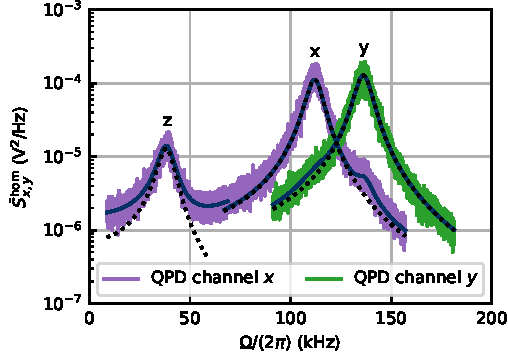
\includegraphics[trim=0cm 0cm 0cm 0cm, width=86mm]{imgs/SI_calibration_078.pdf}
    \caption{Power spectral density $\bar{S}^\mathrm{hom}_{x, y}$ recorded by the $x$ (horizontal, in purple) and $y$ (vertical, in green) channels of the QPD signal, acquired at \SI{9.6}{\milli\bar}. The solid blue lines show simultaneous fits of the peaks associated with the $x$, $y$ and $z$ particle motion for both QPD channels. Dotted lines represent the single oscillator model components of the global fit.
    }\label{fig:PSDhighPressures}
\end{figure}
%
The particle motion is encoded in the position-dependent phase imprinted onto the inelastically scattered light, which interferes with the tweezer and can be read-out interferometrically using a quadrant photodetector.
%
The horizontal ($x$) and vertical ($y$) motion can be efficiently detected on the corresponding differential channels of the QPD (top-down and left-right).
%
The longitudinal ($z$) motion modulates the global intensity of the transmitted tweezer beam, thus should not be seen on the sum channel of the QPD.
%
Nevertheless, imperfections in the alignment of the collection lens and in the detector electronics allows a sufficient portion of the z-motion signal to leak in both differential channels.
%
Here, we used the horizontal (vertical) QPD channel to read out the $x$ and $z$ ($y$) particle motion.

To convert the QPD signal from voltage to displacement units we follow the standard calibration procedure outlined in \cite{Hebestreit2018calibration}.
%
At high pressures, each motional degree of freedom is at thermal equilibrium with the surrounding gas at room temperature $T_\text{gas} = \SI{300}{\kelvin}$.
%
Using the equipartition theorem 
%
\begin{equation}\label{eq:equipartition}
    \frac{1}{2} k_\mathrm{B} T_\text{gas}  = \frac{1}{2} m \Omega_{ j}^2 \langle q_{j}^2 \rangle,
\end{equation}
%
where $\Omega_{j}$ and $\langle q_{ j}^2 \rangle$ (in units of m${^2}$) denote the eigenfrequency and displacement variance of the $j$-th translational mode, respectively.
%
The eigenfrequencies can be extracted from the peaks in the power spectral density (PSD) of the signal $s(t)$ recorded by the QPD.
%
The area under each of the peaks in the PSD  provides the variance $\langle s_j^2 \rangle$ (in voltage units) corresponding to the displacement variance for the $j$-th translational mode.
%
Assuming a linear relation between voltage and displacement $\langle q_j^2 \rangle= c^2_j\langle s_j^2 \rangle $ and using Eq.\eqref{eq:equipartition}, allows determining the voltage to displacement calibration factor 
%
\begin{equation}\label{eq:calibration}
    c_j^2 = \langle s_{j}^2\rangle \cdot \frac{m \Omega_{j}^2}{k_\mathrm{B} T_\text{gas}}
    .
\end{equation}
%


The linewidth $\gamma$ of the peaks in the PSD provides the mechanical damping rate of the particle.
%
Since the damping rate depends on the gas pressure and on particle radius $R$, it is possible to deduce $R$ from the measured damping rate \cite{Hebestreit2018calibration}
%
\begin{equation}
    R = 0.619 \frac{9}{\sqrt{2\pi} \rho_\mathrm{part.}} \sqrt{\frac{M}{N_A k_\mathrm{B} T_\mathrm{gas}} } \frac{P_\mathrm{gas}}{\Gamma},
\end{equation}
%
where $N_A$ is the Avogadro number, $\rho_\mathrm{NP} = \SI{2200}{\kilo\gram}/\SI{}{\meter\cubed}$ the density of silica, $M = \SI{28.97e-3}{\kilo\gram}/\SI{}{\mole}$ the molar mass of air, and $P_\mathrm{gas}$ the gas pressure. 
%
From the particle radius and the mass density $\rho_\mathrm{NP}$ one finally obtains its mass $m$.


Figure~\ref{fig:PSDhighPressures} shows the power spectral density (PSD) obtained from a 1-second time trace of the QPD signals acquired at a pressure of $\SI{9.6}{\milli\bar}$.
%
The particle’s motion along each axis is modelled using the transfer function of a damped harmonic oscillator, $\mathcal{L}_j(\omega) \propto |\Omega^2 - \omega^2 - i\omega\gamma|^{-2}$.
%
Because the tails of the peaks in the PSD partially overlap, we perform simultaneous fits of neighbouring peak pairs (solid dark lines) to more accurately estimate the relevant parameters.
%
From these fits, we extract the individual peak areas, linewidths $\gamma_j$, and central frequencies $\Omega_j$.
%
Dotted lines represent the individual oscillator components of the combined fits.
%
Table~\ref{tab:calibration} summarizes the results of our analysis.
%
\begin{table}[htb]
\centering
 \begin{tabular}{c c c c c c}
 & $\Omega_{ j}/(2\pi)$ & $c_j$ & $\gamma_j/(2\pi)$ & $m$ & $R$\\[0.5ex] 
    & [\SI{}{\kilo\hertz}] & [\SI{}{\volt}/\SI{}{\micro\meter}] & [\SI{}{\kilo\hertz}] & [\SI{}{\femto\gram}] & [\SI{}{\nano\meter}] \\ 
 \hline\hline
\multirow{3}{*}{\begin{tabular}{c|} $x$ \\ $y$ \\ $z$\end{tabular}}
 & 111.99(2) & 19(5) & 9.43(4) & 1.9(9) & 59(8) \\
 & 136.38(3) & 24(6) & 9.18(4) & 1.7(7) & 57(8) \\
 & 38.36(3) & 2.2(6)  & 8.87(4)  & 2.0(8) & 60(8) \\[1ex]
 \end{tabular}
\centering
\caption{Calibration factors $c_j$, eigenfrequencies $\Omega_{j}$ and linewidths $\gamma_j$ extracted at $P=\SI{9.6}{\milli\bar}$, for the nanoparticle used in all free fall experiments with $\tau < \SI{180}{\micro\second}$. Each degree of freedom  provides independent estimates the particle's mass $m$ and radius $R$.
}\label{tab:calibration}
\end{table}

The free fall protocols are executed at $\approx \SI{3e-6}{\milli\bar}$, after initializing each mode into a cold thermal state with effective temperature $T_\text{0, j} \ll \SI{300}{\kelvin}$ through parametric feedback cooling (PFC).
%
We calculate the effective temperatures by comparing the area under the PSD of each mode under PFC with the area of the peaks in the reference PSD where the particle was at thermal equilibrium with the background gas.
%
In the main text we also state the mechanical damping rate $\gamma$ at base pressure extrapolated from the values measured at $10~\mathrm{mBar}$, assuming a linear scaling with pressure \cite{Hebestreit2018calibration}. 


\section{Data Analysis}\label{app:DataAnalysis}

The photocurrent recorded by the QPD detector contains the signal encoded in the position-dependent phase of the scattered field, along with technical noise and shot noise originating from the granular nature of the optical field.
%
To extract information about the particle's motion, we process the raw trajectories from each repetition of the free-fall experiment offline using a second-order bandpass filter.
%
This method preserves the relevant signal while suppressing excess noise outside the signal’s bandwidth.
%
The X (horizontal) and Y (vertical) channels of the QPD are used to infer the oscillator’s motion along the X–Z and Y axes, respectively.


In the frequency domain, the transfer function of the filter used to estimate the position signal has two poles at $\omega = 4i\Gamma_\text{f} \pm \sqrt{\Omega_\text{j}^2 - 16\Gamma_\text{f}^2}$ and one zero at $\omega = 0$.
%
Here, $\Omega_\text{j}$ denotes the resonance frequency of each mechanical mode, and $\Gamma_\text{f}/2\pi = 0.5~\mathrm{kHz}$. 
%
The filter used to extract the momentum signal shares the same poles but has no zero.
%
These expressions can be derived from the Kalman filter formalism in the limit where the conditional state covariance matrix $\vb{\Sigma_c} = \mathrm{diag}(V_n, V_n)$ is diagonal \cite{Wiseman2009, Meng2020}.
%
This limit is valid when the measurement efficiency is very low, as is the case here (approximately $0.5\%$).
%
We also introduce the quantity $\Gamma_\text{f} = V_n \Gamma_\text{m}$, where $\Gamma_\text{m}$ and $V_n$ denote the measurement rate and estimation noise, respectively.

To process each single-shot trajectory corresponding to one repetition of the experiment, we first compute the power spectral density (PSD) of the photocurrent before and after the free fall.
%
From the centroid of the peaks in the PSD, we determine the oscillation frequencies for the initialization ($\Omega_\text{init}$) and measurement ($\Omega_\text{meas}$) phases of the protocol.
%
These frequencies may differ due to state expansion, as the nanoparticle can explore regions where Duffing nonlinearities become significant (see Section~\ref{app:Duffing}).

Following recapture, the softening of the optical potential can induce frequency shifts as large as $5~\mathrm{kHz}$ for the y mode.
%
The fraction of the signal redistributed into mixing and higher-order sidebands remains on the order of a few percent.
%
Additionally, the oscillation amplitude—and hence the relative frequency shift—varies on timescales comparable to the inverse of the oscillator damping rate, $\gamma^{-1}$, which are much longer than the timescales relevant for inferring the oscillator’s state. 
%
This justifies the use of a single bandpass filter with a fixed carrier frequency for state estimation.

We then apply the filter centered at $\Omega_\text{init}$ (or $\Omega_\text{meas}$) forward (or backward) in time to the trajectory.
%
The forward-filtered trajectory characterizes the particle’s state before free fall, while the backward-filtered trajectory does so after free fall. 
%
This approach avoids artifacts arising from transients in the QPD signal during the laser on/off transitions.
%
We repeat this procedure independently for each axis of motion.

Figure~\ref{fig:FilteredPSDs} shows the power spectrum of the raw and filtered Y signals before and after one realization of the free-fall experiment.
%
\begin{figure}[t]
		\centering
		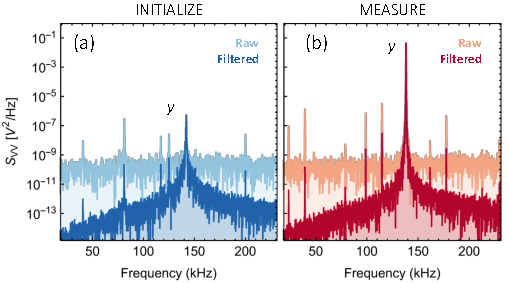
\includegraphics[width=116mm]{imgs/FigS2_FilterPSD.pdf}
    \caption{Power spectral density (PSD) of the raw and filtered QPD-y signal for a representative experimental realization with $\tau = 0.13~\mathrm{ms}$. Panels (a) and (b) display the PSDs recorded during the \textit{initialize} and \textit{measure} phases of the experimental sequence, respectively.}
    \label{fig:FilteredPSDs}
\end{figure}
%
By ensemble-averaging the trajectories over multiple repetitions of the experiment and converting the signals from volts to meters according to the calibration procedure described in Section~\ref{app:calibration}, we obtain the mean displacement at recapture, see Fig.~2(a–c) in the main text.

Under parametric feedback cooling, the effective temperature to which the particle is initialized can fluctuate between realizations. To avoid artifacts in the analysis, we normalize all relevant quantities to those of the initial state.
%
From the final $1.0~\mathrm{ms}$ of the estimated position and momentum signals prior to free fall, we infer the initial state's phase-space distribution, as well as its position variance ($q_0^2$) and momentum variance ($p_0^2$). For each filtered trajectory, we then extract the particle’s position and momentum at recapture and normalize them to $q_0$ and $p_0$, respectively.

From the ensemble of realizations, we compute the second moments of the normalized position ($\tilde{q} = q/q_0$) and momentum ($\tilde{p} = p/p_0$), thereby estimating the average energy stored in the oscillator at recapture in units of the initial state energy, $k_B T_0$ (see Fig.~2(d) in the main text).
%
Finally, using the rescaled phase-space samples at recapture in $(\tilde{q}, \tilde{p})$ coordinates, we estimate the state covariance matrix, whose entries directly yield the parameters $\xi_q$ and $\xi_p$.
%
\begin{figure}[t]
		\centering
		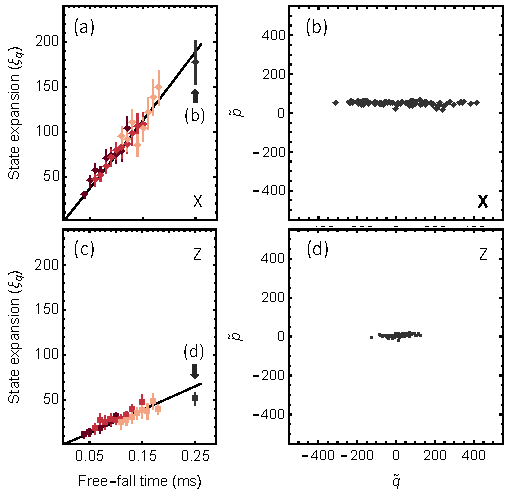
\includegraphics[width=100mm]{imgs/FigS3_ExtendedDatasetFig3.pdf}
    \caption{(a,c) Expansion factor as a function of free fall-time for the $x$ and $z$ axes respectively. The black line is the theory prediction without any free fitting parameters. (b,d) Sampling of phase-space distribution at recapture associated to the $x$ and $z$ motion of the nanoparticle, respectively.
    }
    \label{fig:Extended_datasetFig3}
\end{figure}

\section{Extended dataset}~\label{app:Extended_datasetFig3}
%
We present complementary results for the analysis of the expansion factor and phase space distribution of the particle along the X and Z axes of motion at recapture. 
%
Figure~\ref{fig:Extended_datasetFig3}(a,c) shows the measured expansion factor $\xi_q$ as a function of the free fall time for the particle motion along the $x$ and $z$ axes, respectively. 
%
Error bars correspond to $2\sigma$ standard confidence intervals. 
%
Figure~\ref{fig:Extended_datasetFig3}(b,d) shows the reconstructed phase-space distribution at recapture corresponding to the largest free fall time for the $x$ and $z$ motion, respectively.

\section{Nonlinearity of the optical trap}\label{app:Duffing}


The gradient force in an optical tweezer is approximately linear only for particle displacements that are small compared to the focal spot size.
%
In practice, the trapping potential is governed by the intensity profile of the laser beam, which is Gaussian.
%
Expanding the Gaussian potential in a Taylor series truncated at fourth order, one finds that the nonlinear restoring force acting on the trapped particle yields a displacement-dependent oscillation frequency 
%
\begin{equation}\label{eq:duffing}
\Omega_j = \Omega_{0, j} \left( 1 + \frac{3}{4} \sum_{i = x, y, z} \xi_{ji} \langle q_i^2 \rangle \right).
\end{equation}
%
For a Gaussian beam, the Duffing tensor is \cite{hebestreit2017thermal}:
%
\begin{equation}\label{eq:DuffingTensor}
\boldsymbol{\xi} =
\begin{pmatrix}
\xi_{xx} & \xi_{xy} & \xi_{xz} \\
\xi_{yx} & \xi_{yy} & \xi_{yz} \\
\xi_{zx} & \xi_{zy} & \xi_{zz}
\end{pmatrix}
\approx
\begin{pmatrix}
\xi_{x} & \xi_{y} & \xi_{z} \\
\xi_{x} & \xi_{y} & \xi_{z} \\
2 \xi_{x} & 2 \xi_{y} & \xi_{z}
\end{pmatrix},
\end{equation}
%
where $\xi_j = -2/w_j^2$ is inversely proportional to the square of the trap diameter $w_j$ along the respective axis.

After a free fall, the oscillation amplitude increases due to the gain in kinetic energy and, more significantly, due to the increased position uncertainty.
%
This results in a redshift of the eigenfrequencies of all three center-of-mass (COM) modes at recapture.
%
\begin{figure}[t]
\centering
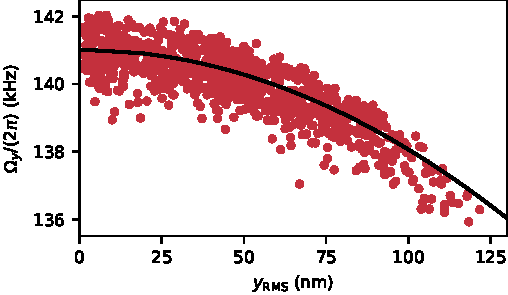
\includegraphics[trim=0cm 0cm 0cm 0cm, width=80mm]{imgs/duffing_y_red.pdf}
\caption{Oscillation frequency versus root-mean-square (RMS) oscillation amplitude along the gravity axis $y$. 
%
The dark line is a fit to Eq.~\eqref{eq:duffing}, fixing the variances along $\langle x^2 \rangle$ and $\langle z^2 \rangle$ to their average value across all experiment repetitions.
}
\label{fig:Duffing}
\end{figure}

Figure~\ref{fig:Duffing} shows the oscillation frequency $\Omega_y$ at recapture as a function of the root-mean-square amplitude $y_\mathrm{RMS}$ along the vertical axis.
%
The latter is computed as the square root of the displacement variance, $y_\mathrm{RMS} = \sqrt{\langle y^2 \rangle}$.
%
The variance is estimated by integrating the PSD of the signal after recapture over a \SI{5}{\kilo\hertz} bandwidth around each mode, then converting the result into displacement units using the calibration factor extracted in Section~\ref{app:calibration}.
%
Each data point corresponds to a free-fall experiment performed between tweezer positions displaced by approximately \SI{100}{\nano\meter}, with free evolution times ranging from \SI{60}{\micro\second} to \SI{150}{\micro\second}.
%
As the oscillation amplitude grows to values comparable to the trap size, the eigenfrequency decreases—consistent with the softening characteristic of the Duffing nonlinearity for Gaussian beams.

The solid line in Fig.\ref{fig:Duffing} represents a fit to Eq.\eqref{eq:duffing}, treating the three tensor components $\xi_j$ as free parameters, while fixing the variances along the $x$ and $z$ axes to their average values across all experiment repetitions: $\langle q_x^2 \rangle = (\SI{38}{\nano\meter})^2$ and $\langle q_z^2 \rangle = (\SI{63}{\nano\meter})^2$.
%
From the fit, we extract the Duffing coefficients:
%
$\xi_{x} = \SI{-1.72(3)}{\micro\meter^{-2}}$,
$\xi_{y} = \SI{-2.78(2)}{\micro\meter^{-2}}$, and
$\xi_{z} = \SI{-0.32(1)}{\micro\meter^{-2}}$.
%
Since $\xi_j = -2/w_j^2$, we can estimate the optical beam waist and Rayleigh range:
$w_x = \SI{1.08(1)}{\micro\meter}$,
$w_y = \SI{0.85(1)}{\micro\meter}$, and
$w_z = \SI{2.50(4)}{\micro\meter}$.
%
The fact that $w_x > w_y$ is consistent with the linear $x$-polarization of the tweezer. All extracted values are in good agreement with those predicted by ray-tracing simulations for the nominal trapping lens geometry.


\bibliographystyle{apsrev4-1}
\bibliography{biblioFF.bib} 



\end{document}
